\section{ADC Unit}

The analog/digital converter unit is one of the most complicated and powerful units implemented in the project.

The unit can measure the voltage on an input pin, either as its immediate value, or averaged with exponential forgetting. The smoothing formula is ($y$--averaged output, $t$--sample number, $k$--smoothing factor, $u$--raw measured value):

\begin{equation}
	y[t] = (1-k)\cdot y[t-1] + k\cdot u[t]
\end{equation}

Isochronous sampling is available as well: it is possible to capture a fixed-length block of data on demand, or as a response to a triggering condition on any of the enabled input pins. The \gls{ADC} must continuously sample the inputs to make the averaging and level based triggering possible, which is implemented using \gls{DMA}; as a consequence, a pre-trigger buffer is available that can be read together with the block of samples following a trigger (\cref{fig:adc_dma}). The \gls{ADC} unit can also be switched to a continuous streaming mode, a block capture which continues indefinitely, until the host decides to stop the stream.

It is possible to activate any number of the 16 analog inputs of the \gls{ADC} peripheral simultaneously, together with the internal input channels. The maximum continuous sampling frequency, which reaches 70\,ksps with one channel, lowers with an increasing number of enabled channels, as the amount of data to transfer host increases. Those high speeds are achievable in shorter block captures, taking advantage of the (configurable) data buffer. An ongoing capture may be terminated by the unit after the buffer is exhausted.

\begin{figure}[h]
	\centering
	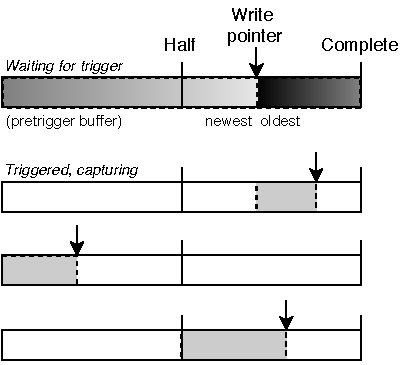
\includegraphics[scale=1]{img/adc-dma-buf.pdf}
	\caption[Principle of DMA-based ADC sampling]{\label{fig:adc_dma}Principle of DMA-based ADC sampling. The buffer is continually filled with new samples; when the triggering condition is hit, the historical records from the buffer are sent as a pre-trigger buffer, and a block capture begins. The following samples are sent to the host when either half of the buffer is filled, or the required number of samples have been sent. The sampling never stops, ensuring a pre-trigger buffer is always ready.}
\end{figure}

\subsection{ADC Configuration}

\begin{inicode}
[ADC:adc@8]
# Enabled channels, comma separated
#  0  1  2  3  4  5  6  7    8  9   10 11 12 13 14 15   16    17
# A0 A1 A2 A3 A4 A5 A6 A7   B0 B1   C0 C1 C2 C3 C4 C5   Tsens Vref
channels=16

# Sampling time (0-7)
sample_time=2
# Sampling frequency (Hz)
frequency=1000

# Sample buffer size
# - shared by all enabled channels
# - defines the maximum pre-trigger size (divide by # of channels)
# - captured data is sent in half-buffer chunks
# - buffer overrun aborts the data capture
buffer_size=256

# Enable continuous sampling with averaging
# Caution: This can cause DAC output glitches
averaging=Y
# Exponential averaging coefficient (permil, range 0-1000 ~ 0.000-1.000)
# - used formula: y[t]=(1-k)*y[t-1]+k*u[t]
# - not available when a capture is running
avg_factor=500
\end{inicode}

\subsection{ADC Events}

\begin{cmdlist}
	50 & \cname{TRIGGERED}
	The first event generated when a triggering condition occurs. The payload includes pre-trigger and the transaction continues with a sequence of CAPTURE events sharing the same frame ID. The serial number is incremented with each stream chunk and can be used to detect lost data frames.
	&
	\begin{cmdpld}
		\cfield{u32} pre-trigger length
		\cfield{u8} triggering edge (1--falling, 2--rising, 3--forced)
		\cfield{u8} stream serial number
		\cfield{u16[]} pre-trigger data
	\end{cmdpld}
	\\

	51 & \cname{CAPTURE\_DATA}
	A chunk of sampled data in a stream, block, or a triggered capture. More data will follow.
	&
	\begin{cmdpld}
		\cfield{u8} stream serial number
		\cfield{u16[]} sample data
	\end{cmdpld}
	\\

	52 & \cname{CAPTURE\_END}
	Indicates the end of a multi-part capture. The payload may be empty if there is no more data to send (e.g., a stream had to be unexpectedly closed).
	&
	\begin{cmdpld}
		\cfield{u8} stream serial number
		\cfield{u16[]} sample data
	\end{cmdpld}
\end{cmdlist}


\subsection{ADC Commands}

\begin{cmdlist}
	0 & \cname{READ\_RAW}
	Get the last raw sample from enabled channels.
	&
	\begin{cmdresp}
		\cfield{u16[]} raw values 0--4095
	\end{cmdresp}
	\\

	1 & \cname{READ\_SMOOTHED}
	Get the averaged values from enabled channels. Not available for high sample rates and when disabled.
	&
	\begin{cmdresp}
		\cfield{float[]} smoothed values 0--4095
	\end{cmdresp}
	\\

	2 & \cname{READ\_CAL\_CONSTANTS}
	Read factory calibration constants from the \gls{MCU}'s \gls{ROM}. These are used to calculate real voltage or temperature from the ADC output word. The formulas can be found in Section 13.9 of the STM32F0~reference manual~\cite{f072-rm}.
	&
	\begin{cmdresp}
		\cfield{u16} VREFINT\_CAL (word)
		\cfield{u16}~VREFINT\_CAL\_VDD~(mV)
		\cfield{u16} TS\_CAL1 (word)
		\cfield{u16} TS\_CAL2 (word)
		\cfield{u16} TS\_CAL1\_T (°C)
		\cfield{u16} TS\_CAL2\_T (°C)
		\cfield{u16} TS\_CAL\_VDD (mV)
	\end{cmdresp}
 	\\

	10 &
	\cname{GET\_ENABLED\_CHANNELS}
	Get numbers of all enabled channels (0-based)
	&
	\begin{cmdresp}
		\cfield{u8[]} enabled channel numbers
	\end{cmdresp}
	\\

	11 &
	\cname{GET\_SAMPLE\_RATE}
	Get the current sample rate (in Hz)
	&
	\begin{cmdresp}
		\cfield{u32} requested sample rate
		\cfield{float} achieved sample rate
	\end{cmdresp}
	\\

	20 &
	\cname{SETUP\_TRIGGER}
	Configure the triggering level and other trigger parameters. This command does \textit{not} arm the trigger.
	&
	\begin{cmdreq}
		\cfield{u8} source channel number
		\cfield{u16} triggering level
		\cfield{u8} active edge (1--falling, 2--rising, 3--any)
		\cfield{u32} pre-trigger sample count
		\cfield{u32} post-trigger sample count
		\cfield{u16} hold-off time (ms)
		\cfield{bool} auto re-arm
	\end{cmdreq}
	\\

	21 & \cname{ARM}
	Arm the trigger for capture.
	&
	\begin{cmdreq}
		\cfield{u8} auto re-arm (0, 1, 255--no change)
	\end{cmdreq}
	\\

	22 & \cname{DISARM}
	Dis-arm the trigger.
	& \\

	23 & \cname{ABORT}
	Abort any ongoing capture and dis-arm the trigger.
	& \\

	24 & \cname{FORCE\_TRIGGER}
	Manually trip the trigger, as if the threshold level was reached.
	& \\

	25 & \cname{BLOCK\_CAPTURE}
	Capture a fixed-length sequence of samples.
	&
	\begin{cmdreq}
		\cfield{u32} number of samples
    \end{cmdreq}
    \\

	26 & \cname{STREAM\_START}
	Start a continuous stream of samples
	& \\

	27 & \cname{STREAM\_STOP}
	Stop an ongoing stream
	& \\

	28 & \cname{SET\_SMOOTHING\_FACTOR}
	Set the smoothing factor ($\times10^3$). 1000 corresponds to $k=1$.
	&
	\begin{cmdreq}
		\cfield{u16} smoothing factor 0--1000
	\end{cmdreq}
    \\

	29 & \cname{SET\_SAMPLE\_RATE}
	Set the sampling frequency.
	&
	\begin{cmdreq}
		\cfield{u32} frequency in Hz
	\end{cmdreq}
    \\

	30 & \cname{ENABLE\_CHANNELS}
	Select channels to sample. The channels must be configured in the unit settings.
	&
	\begin{cmdreq}
		\cfield{u32} bit map of channels to enable
	\end{cmdreq}
    \\

	31 & \cname{SET\_SAMPLE\_TIME}
	Set the sample time of the \gls{ADC}'s sample\&hold circuit.
	&
	\begin{cmdreq}
		\cfield{u8} sample time 0--7
	\end{cmdreq}

\end{cmdlist}
